% results.tex
\documentclass[main.tex]{subfiles}
\begin{document}
\chapter{Results} \label{ch:res}

This chapter presents all the results stemming from the experimental procedures described in Chapter \ref{ch:exp}. Additionally, details are provided regarding proper data processing, and the calculations that lead to the definition of the desired failure surface. 

\section{Tensile Tests} \label{sec:tensr}
Performing tensile tests showed that the values of $X_t$ and $Y_t$ were significantly different, in accordance to the literature review presented in Section \ref{ssec:mechPropFFF}. An initial number of 20 samples per orientation was produced, however, multiple specimens failed outside the gage section of the coupon and thus, data originating from these coupons was considered invalid and promptly discarded. The valid results are summarized in Table \ref{tab:tensrtab}. Note that $X_t$ was on average 9.16 MPa higher than $Y_t$, a difference of 22.7\%.
\begin{table} [h]
	\centering
	\caption{Summary of Tensile tests}
\begin{tabular}{ c| c c } 
	\toprule
	\textbf{Information} & $X_t$ & $Y_t$\\
	\midrule
	Average [MPa] & 40.29 & 31.13\\
	Standard Deviation & 0.75 & 0.58\\
	Number of samples & 19 & 12\\
	Lowest measurement [MPa] &39.37  & 29.68\\
	Highest measurement [MPa] &40.90 & 32.08\\
	\bottomrule
\end{tabular}
\label{tab:tensrtab}
\end{table}

The behavior of both sets of samples was completely different. Coupons used to measure $X_t$ clearly showed whitening of the gage section, indicating plastic deformation. Specimens used for $Y_t$ on the other hand generally failed between beads and rarely showed any change in color. Figure~\ref{fig:tensComp} clearly shows the difference in mechanical behavior. Note how the $X_t$ specimen shows a ductile failure, as opposed to brittle breakage for the $Y_t$ sample. Figure \ref{fig:tensSComp} shows both tested samples side by side.
\pagebreak

\begin{figure}[h]
	\center
	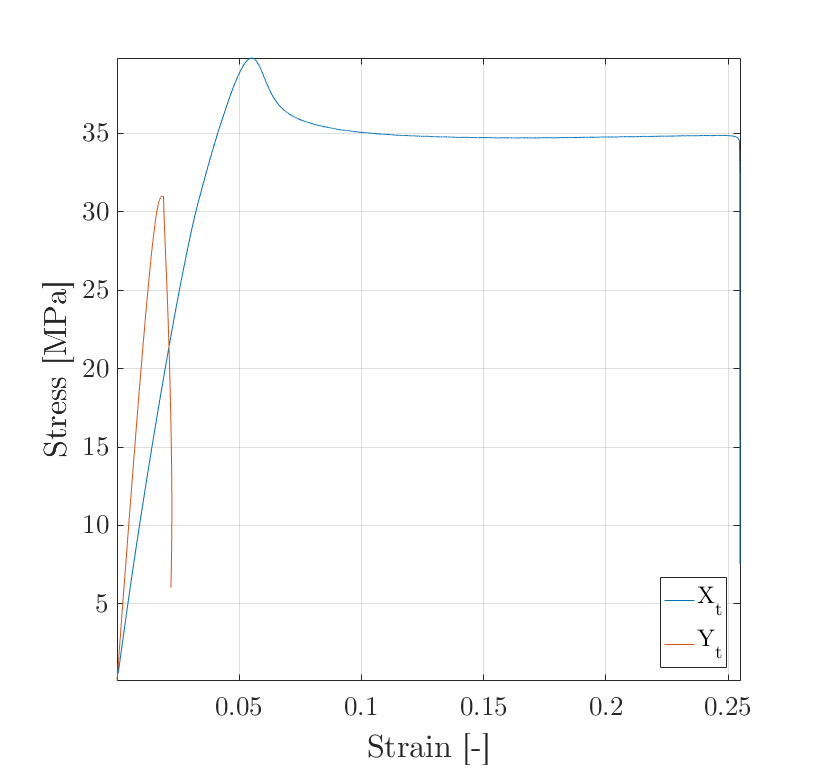
\includegraphics[height=9cm, keepaspectratio]{tenscomp}
	\caption{Comparison of tensile results} \label{fig:tensComp}
\end{figure}

\begin{figure}[!htbp]
	\center
	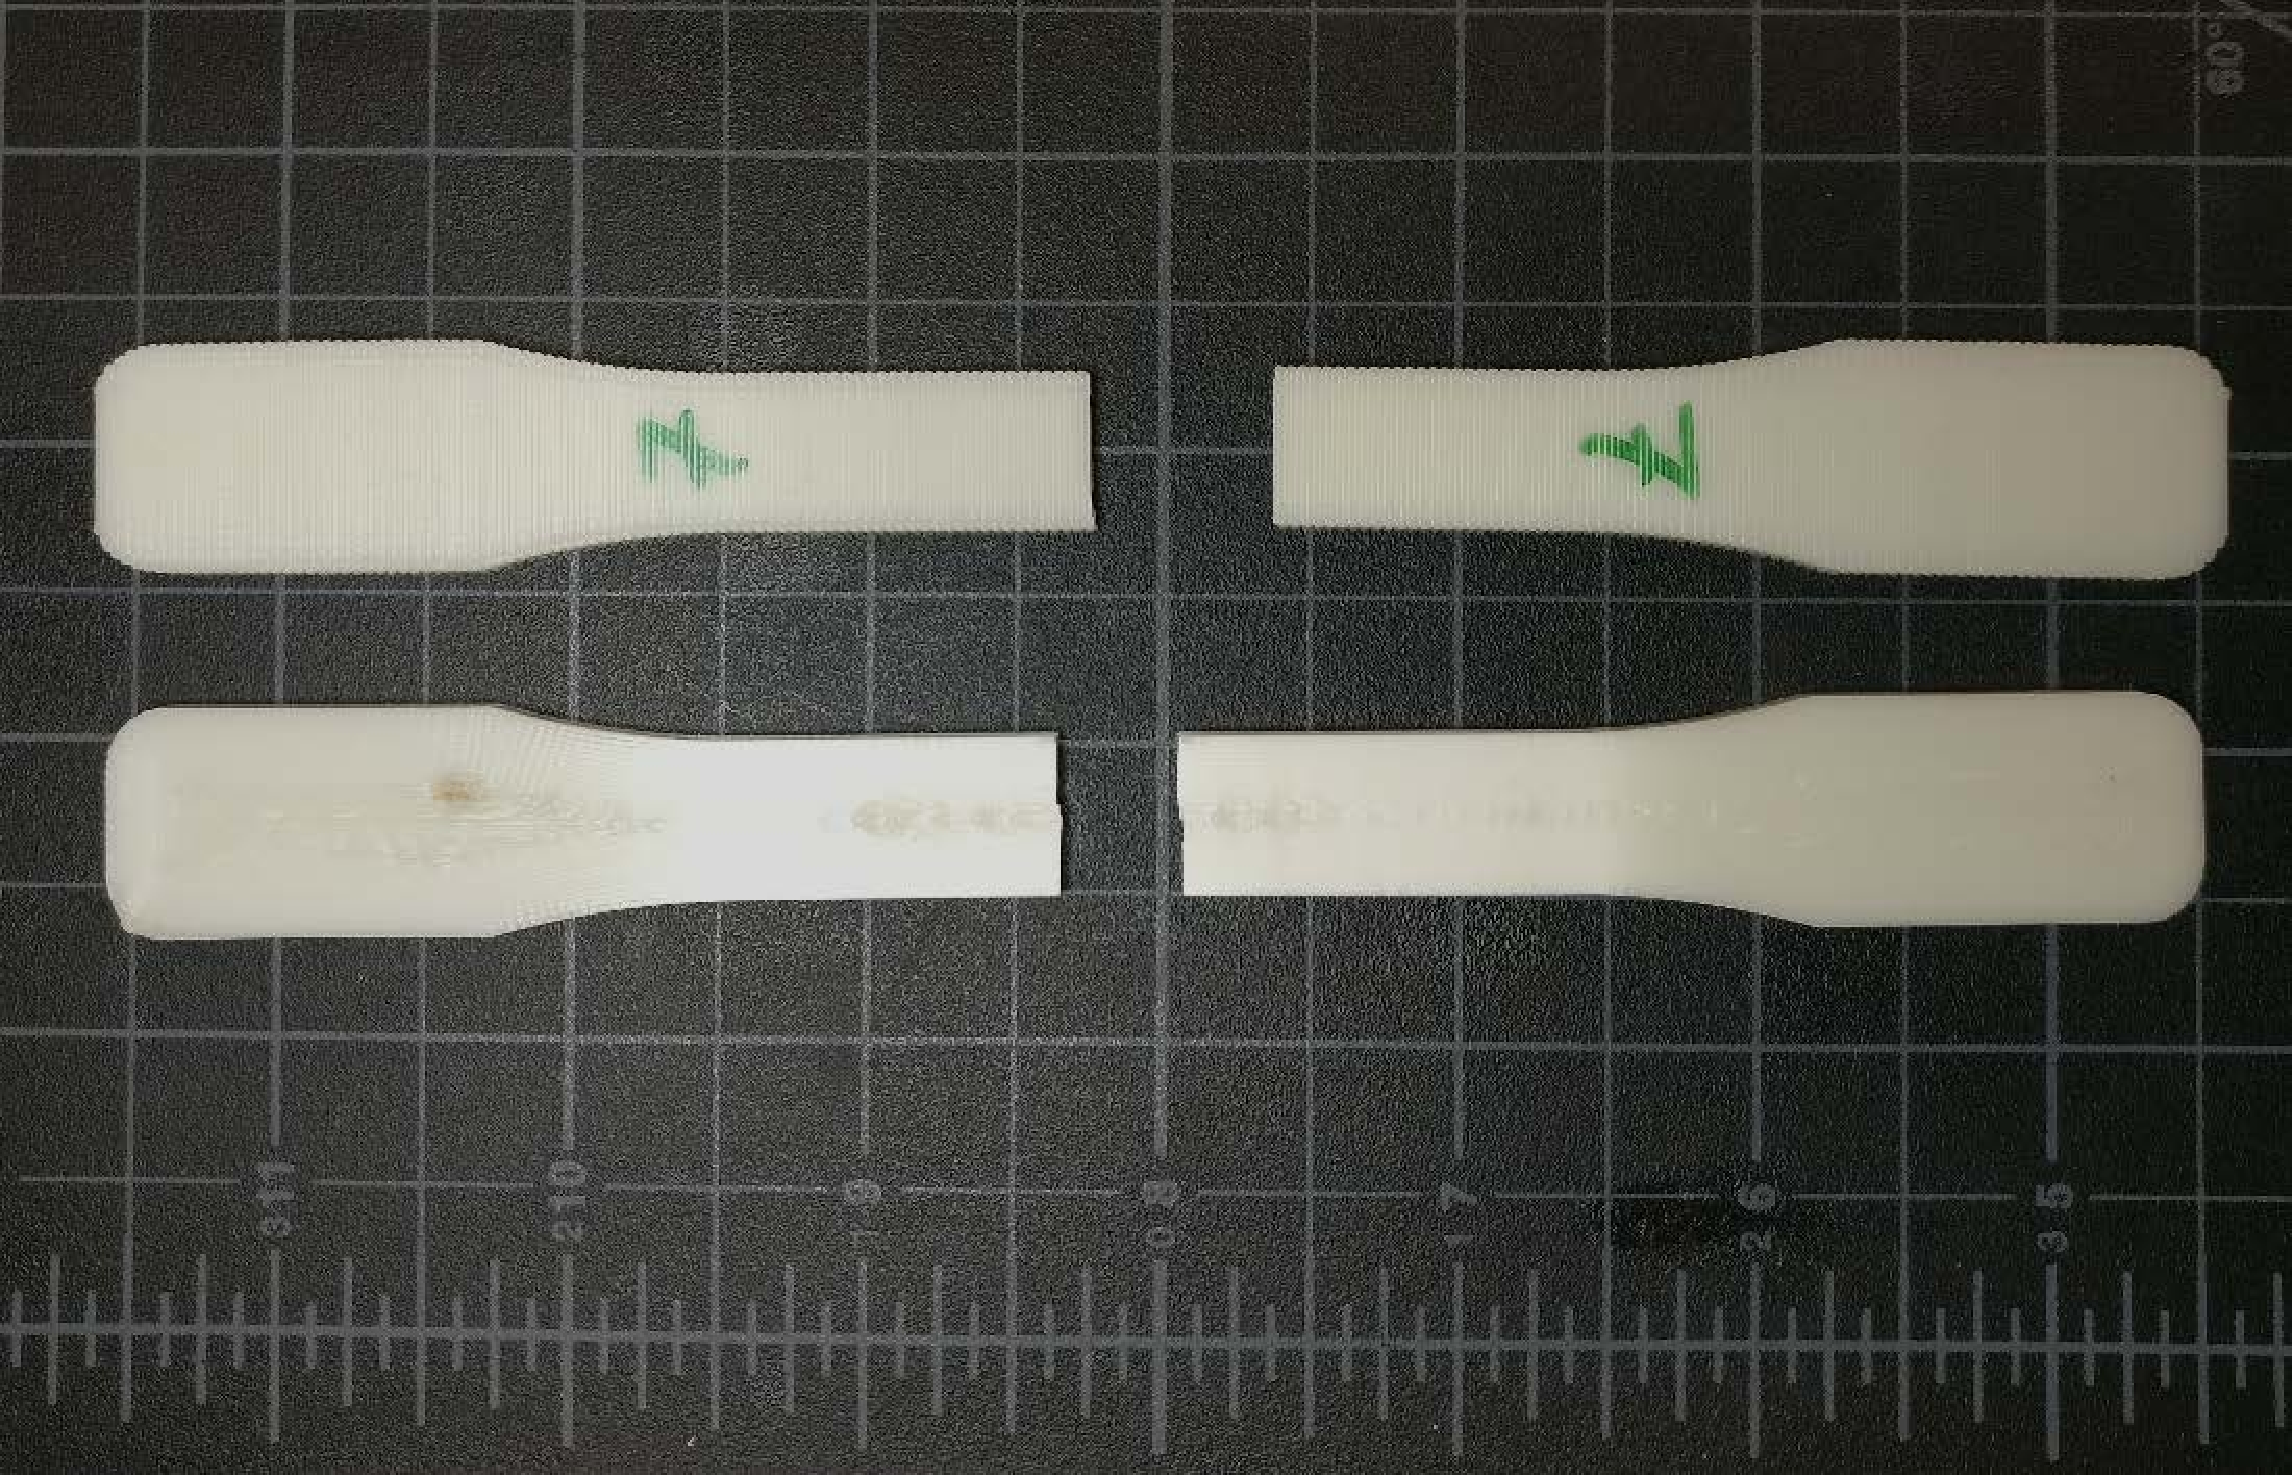
\includegraphics[height=6cm, keepaspectratio]{tenscsomp.pdf}
	\captionsetup{justification=centering} %long caption
	\caption[$X_t$ and $Y_t$ tested samples]{$Y_t$ (top) and $X_t$ (bottom) tested samples. Scale in inches. Note whitening in gage section for $X_t$ specimen.} \label{fig:tensSComp}
\end{figure}

Anderson-Darling tests (ADT) were performed on the results to validate if the data follows a normalized distribution. In the case of $X_t$, the ADT yields a p-value of 0.023. Thus, on a 95\% confidence interval, a normalized distribution can be discarded. This can be seen graphically in the goodness of fit plot, where data points fail to align with the slope that corresponds to a theoretical Gaussian distribution. By contrast, performing the ADT on the $Y_t$ samples fails to reject a normalized distribution using the same confidence interval, offering a p-value of 0.109. %A case could be made for a false negative for $X_t$ and a false positive for $Y_t$, given the relatively small sample size for each data set.
The results from ADT can be seen in Figure \ref{fig:adttens}.

%FIX
\begin{figure}[!htbp]
	\center
	\subfloat[$X_t$ \label{fig:adtxt}]{%
		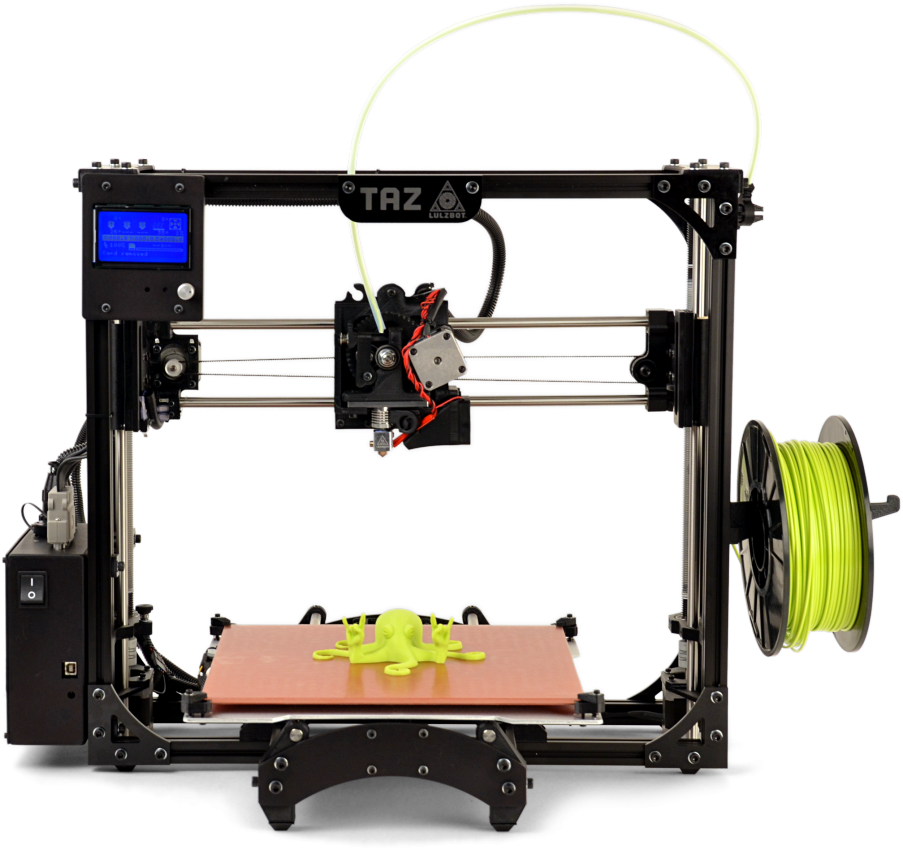
\includegraphics[height=4cm, keepaspectratio]{TAZ_5}
	}
	\hfill
	\subfloat[$Y_t$\label{fig:adtyt}]{%
		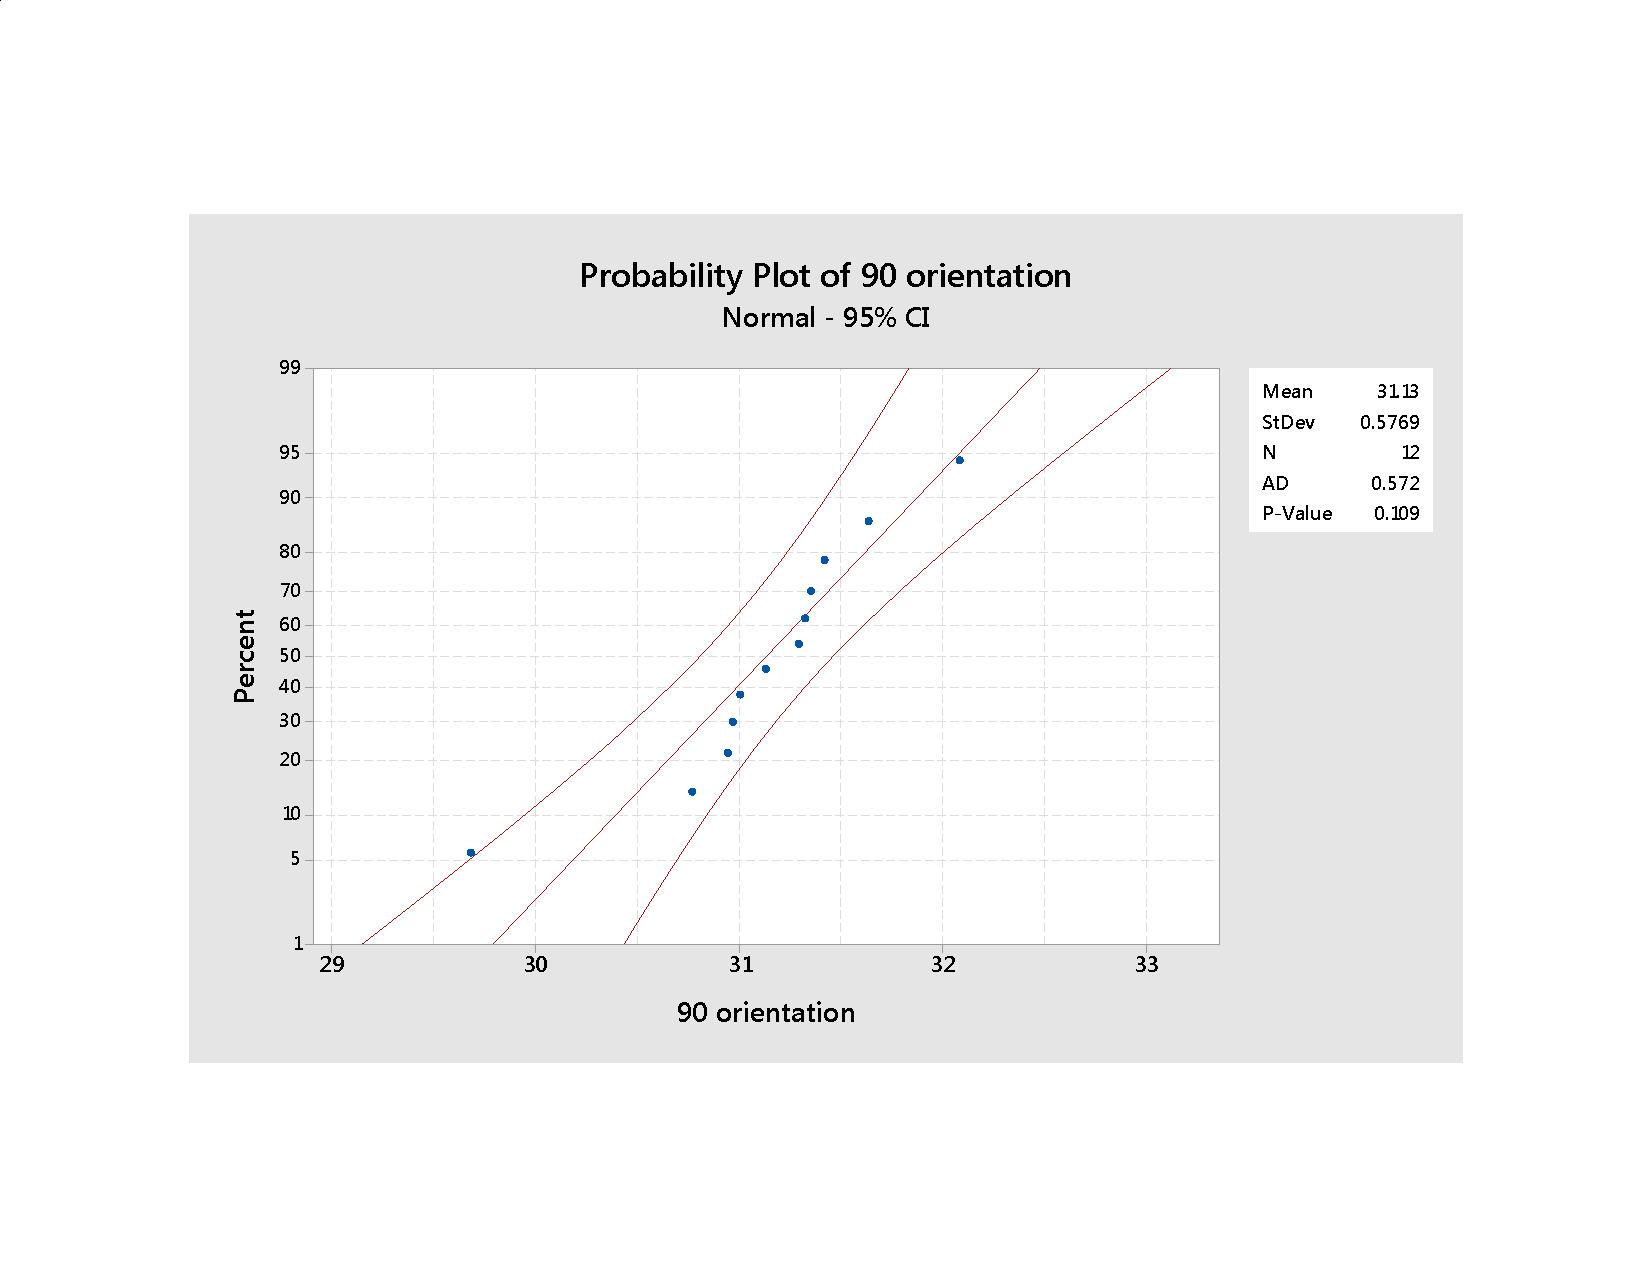
\includegraphics[height=4cm, keepaspectratio]{ADTyt.pdf}
	}
	\caption{ADT results for tensile data} \label{fig:adttens}
\end{figure}
      
\section{Compression Tests} \label{sec:compr}
For the compression tests, a total of 25 samples were produced for each orientation. However, a number of coupons were discarded due to manufacturing defects. Table \ref{tab:comprtab} summarizes the test results.  

\begin{table} [h]
	\centering
	\caption{Summary of Compression tests}%ELABORATE
	\begin{tabular}{ c| c c } 
		\toprule
		\textbf{Information} & $X_c$ & $Y_c$\\
		\midrule
		Average [MPa] &43.91  & 57.96\\
		Standard Deviation &3.23  & 1.81\\
		Number of samples &25  & 22\\
		Lowest measurement [MPa] &37.95 &54.93 \\
		Highest measurement [MPa] &48.87 &61.39 \\
		\bottomrule
	\end{tabular}
\label{tab:comprtab}
\end{table}

Surprisingly, both sets of specimens had different failure behavior. The $Y_c$ samples displayed pure ductile behavior through testing. A clear maximum stress can be observed at the yield point in a stress-strain graph, and all samples showed localized whitening and deformation along the center of the specimen. By contrast, the $X_c$ samples showed a considerably lower yield point, and specimens deformed in a way that formed petal-like structures due to contiguous bead delamination. This difference in mechanical behavior can be seen in Figure \ref{fig:comprComp}, where stress-strain curves for $X_c$ and $Y_c$ are compared. Note the erratic behavior of the $X_t$ sample, caused by delamination of adjacent beads. Figure \ref{fig:CompSComp} shows $X_c$ and $Y_c$ samples side by side post testing, where the different failure behavior becomes evident. 

\begin{figure}[!htbp]
	\center
	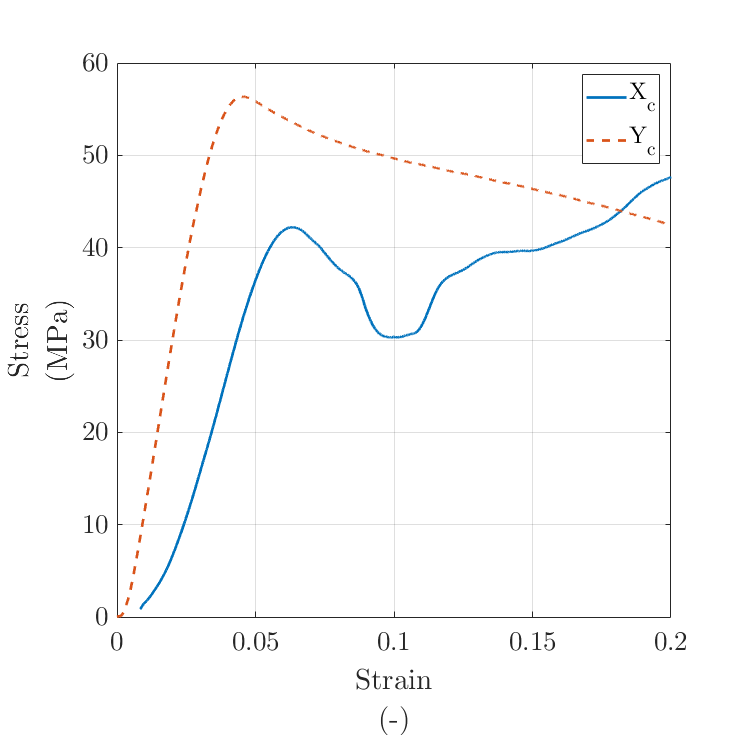
\includegraphics[height=9cm, keepaspectratio]{compresscomp}
	\caption{Comparison of compression results} \label{fig:comprComp}
\end{figure}  

\begin{figure}[!htbp]
	\center
	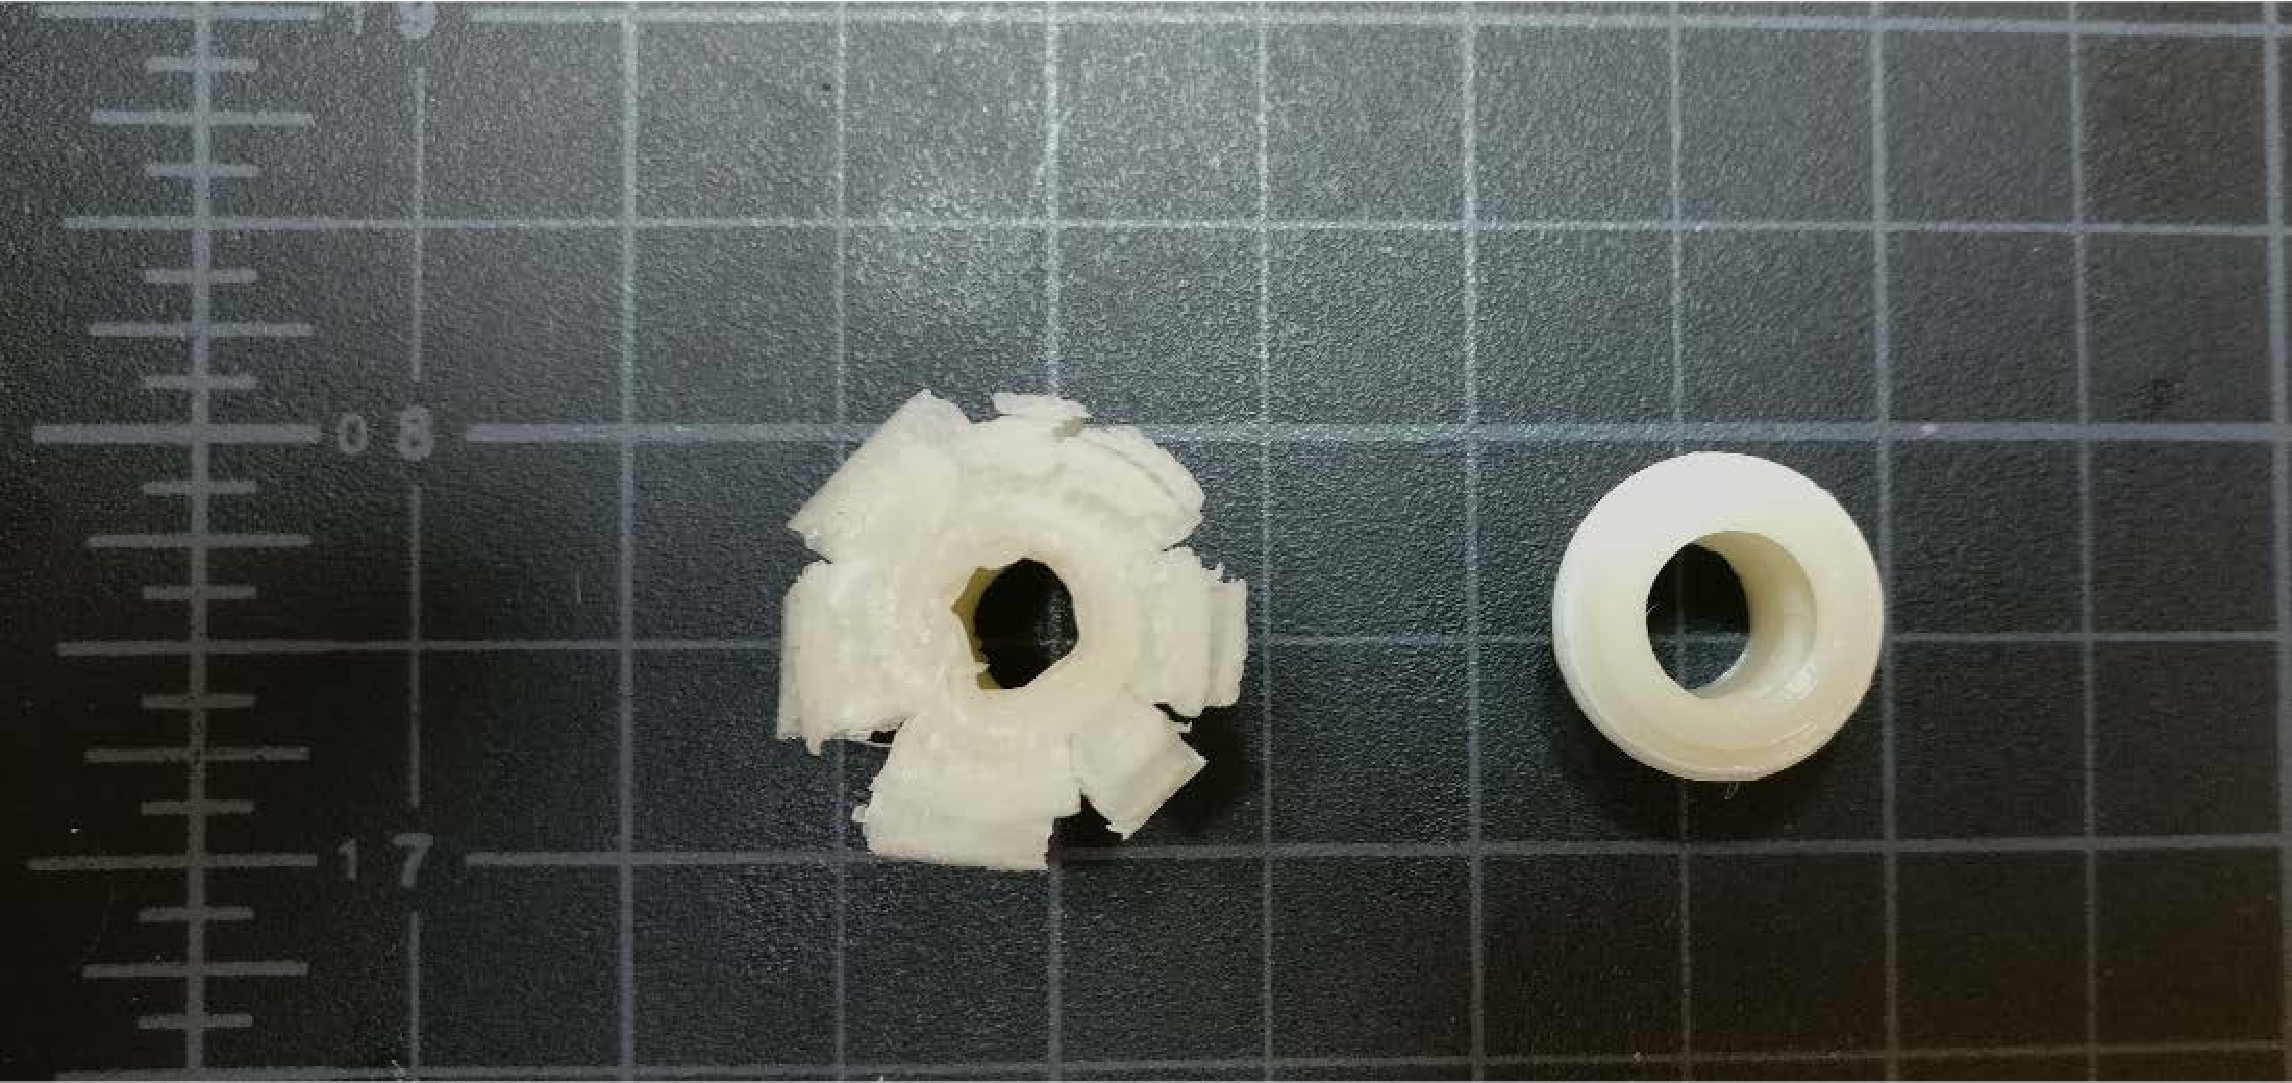
\includegraphics[height=6cm, keepaspectratio]{compscomp.pdf}
	\captionsetup{justification=centering} %long caption
	\caption[$X_c$ and $Y_c$ tested samples]{$X_c$ (left) and $Y_c$ (right) tested samples. Scale in inches. Note petal-like structure of $X_c$ sample.} \label{fig:CompSComp}
\end{figure}

Performing ADT on the data reveals a p-value of 0.072 for $Y_c$, and 0.056 for $X_c$, thus, normalized distributions cannot be discarded on a 95\% confidence interval. %ELABORATE
\section{Torsion Tests} \label{sec:torsr}
\subsection{45$^\circ$ orientation} \label{ssec:45r}
A total of 30 samples were produced with a 45$^\circ$ bead orientation, divided evenly for tests in positive and negative shear. As was the case for tensile and compressive tests, a number of specimens had to be discarded due to undesired behavior during testing. A common problem was delamination of the grips, thus requiring the data to be discarded. 

Results showed significant difference in behavior depending on the direction of the applied torque. The $S_{45p}$ samples showed a completely brittle behavior, with fracture occurring between beads, as opposed to ductile failure in the center of the specimen for the $S_{45n}$ coupons. This resulted in an average difference of 6.3 MPa between both sets of data. Results are summarized in Table \ref{tab:tors45r} and a graph comparing the behavior of both sets of samples can be seen in Figure \ref{fig:45comp}. Note how the positive shear sample fails at low angles in a completely brittle manner.

\begin{table} [h]
	\centering
	\caption{Summary of 45$^\circ$ torsion tests}
\begin{tabular}{ c| c c } 
	\toprule
	\textbf{Information} & $S_{45p}$ & $S_{45n}$\\
	\midrule
	Average [MPa] & 20.80 & 27.13\\
	Standard Deviation & 2.50 & 0.50\\
	Number of samples & 9 & 9\\
	Lowest measurement [MPa] &17.21  & 26.59\\
	Highest measurement [MPa] &24.61 & 28.17\\
	\bottomrule
\end{tabular}
\label{tab:tors45r}
\end{table}

\begin{figure}[!htbp]
	\center
	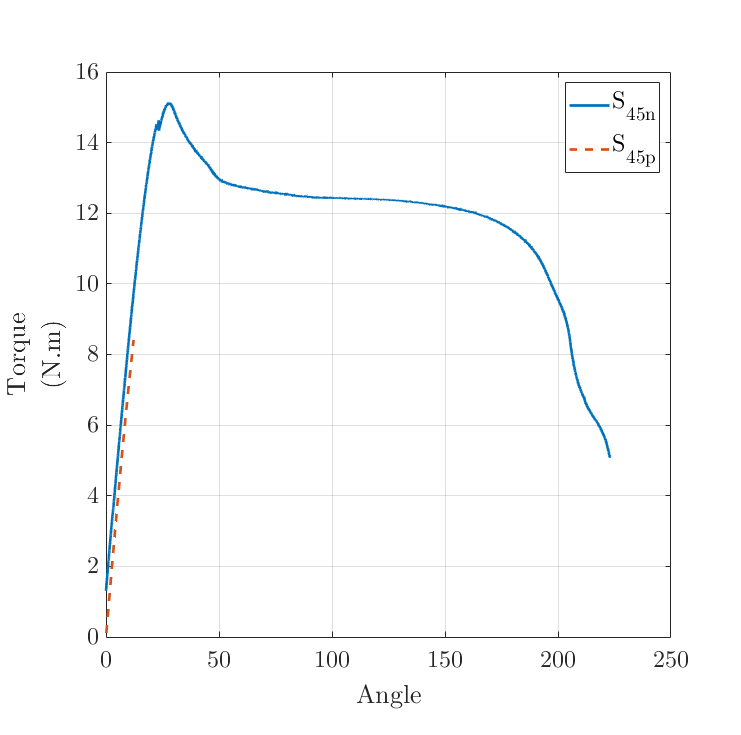
\includegraphics[height=9cm, keepaspectratio]{comp45t}
	\caption{Comparison of 45$^\circ$ torsion results} \label{fig:45comp}
\end{figure}

\begin{figure}[!htbp]
	\center
	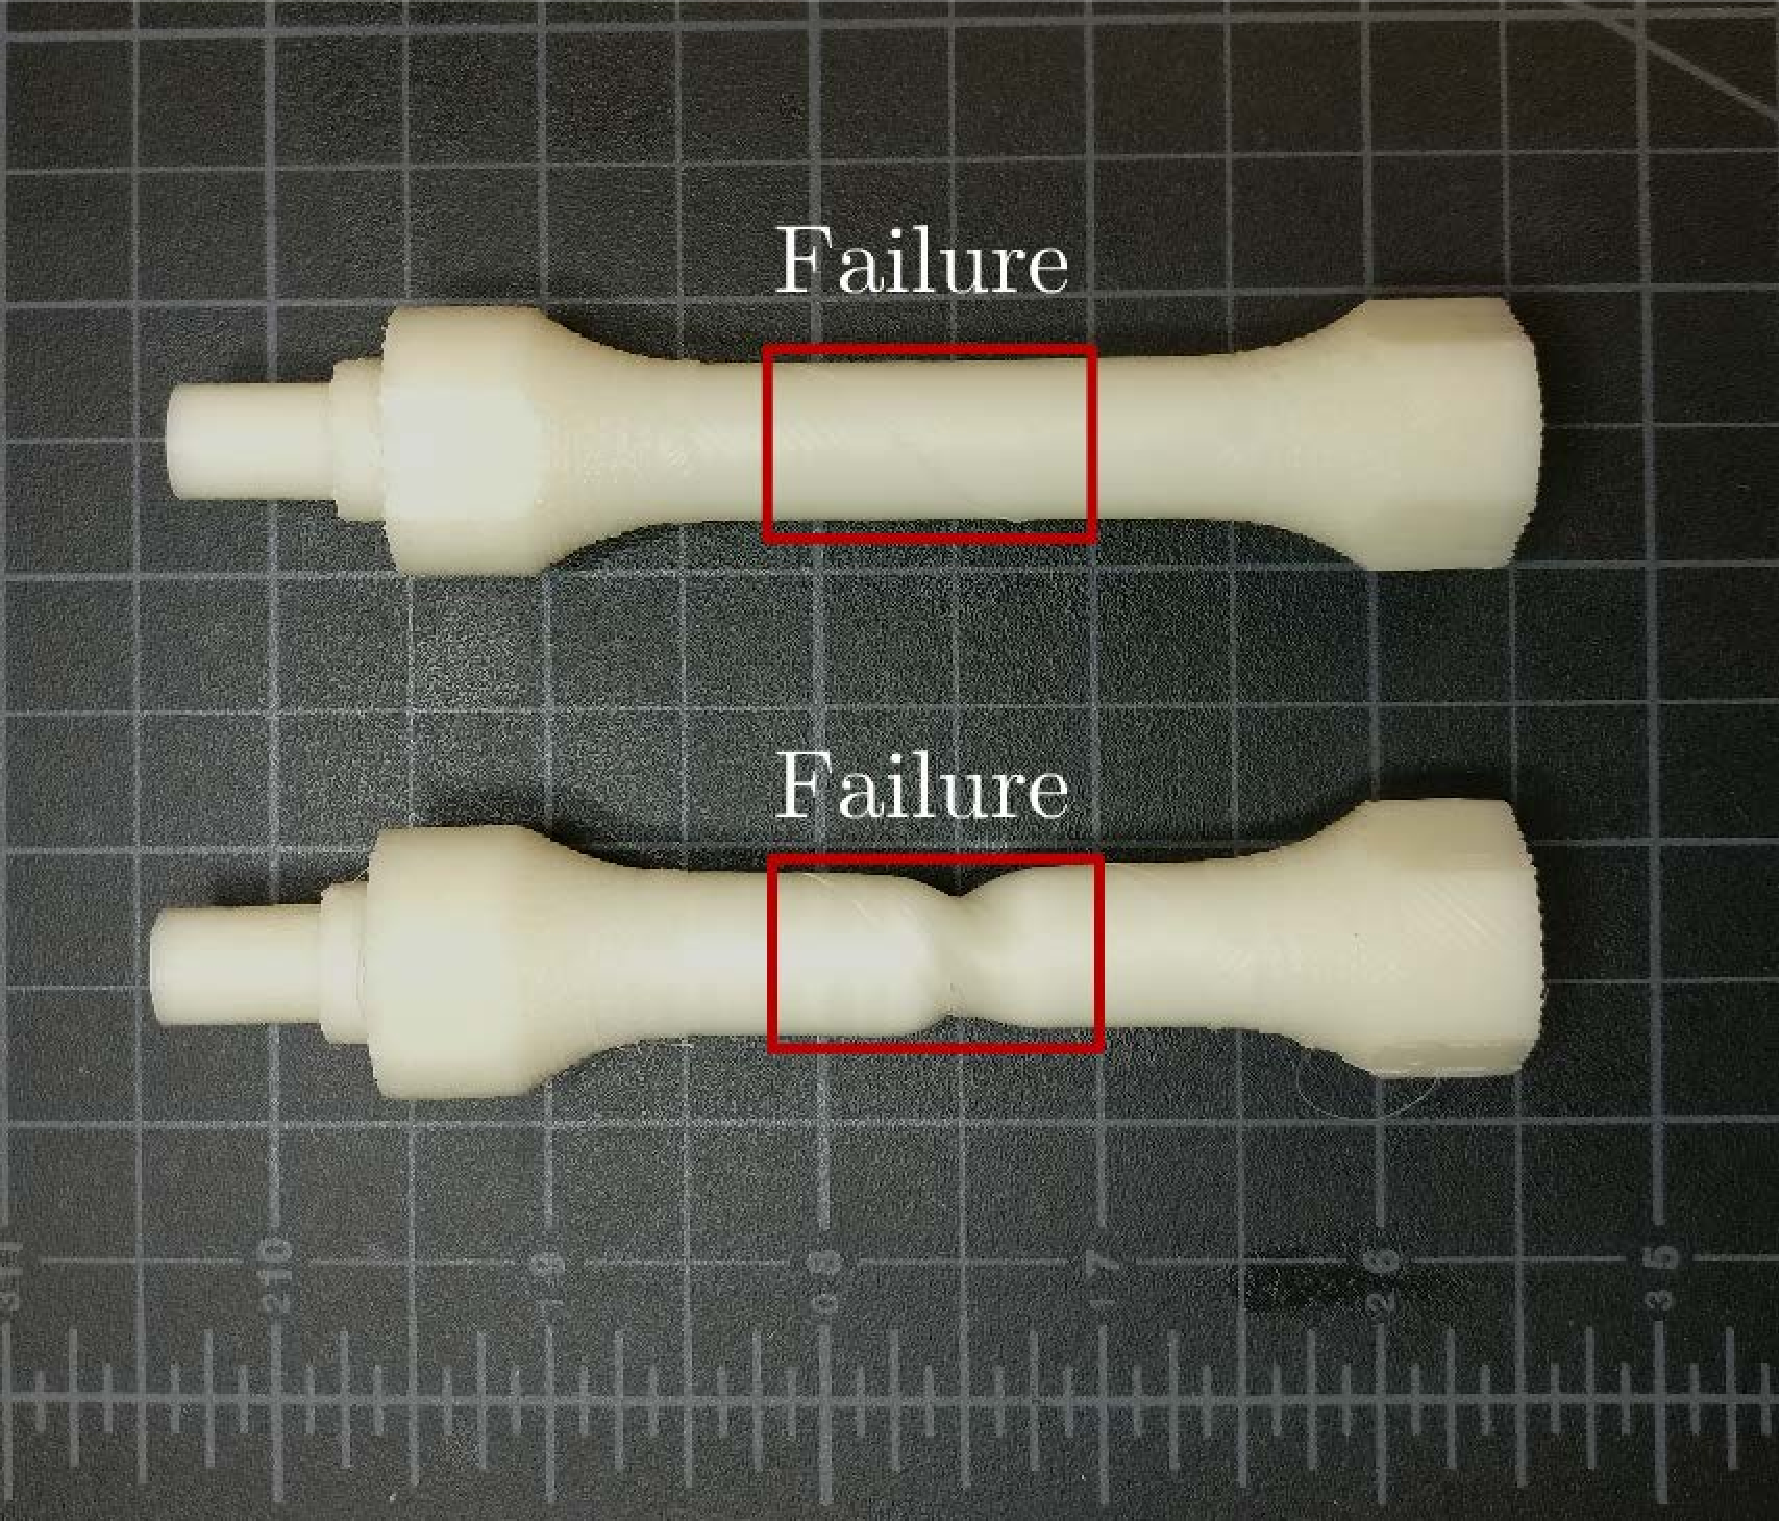
\includegraphics[height=7cm, keepaspectratio]{t45scomp}
	\captionsetup{justification=centering} %long caption
	\caption[Comparison of 45$^\circ$ torsion results]{Comparison of 45$^\circ$ torsion samples. Positive shear (top) caused bead delamination and brittle failure, whereas negative shear (bottom) produced plastic deformation of the gage section} \label{fig:45scomp}
\end{figure}
  
\subsection{0$^\circ$ orientation} \label{ssec:0r}
\subsection{90$^\circ$ orientation} \label{ssec:90r}
\section{Combined Loading Tests} \label{sec:clr}
\section{Development of the Failure Surface} \label{sec:fsc}

The failure surface calculations were performed using MATLAB\textregistered~code based on previous work by Obst \emph{et al.} \cite{Obst2018} and the mathematical relations shown in Chapter \ref{ch:oocrit}. This code can be found in Appendix \ref{ch:fsurfcode} for reference.

Calculations were based on the average values obtained from the mechanical tests in order to incorporate a probabilistic approach as developed by Zaitsev, Pashkov and Strelyaev \cite{Zaitsev1975}. In practice, this signifies that the condition $f=1$ in Equation \ref{eq:GKCfinal} is equivalent to a probability of part failure equal to 50\%.

Starting with the $\sigma_{11}$-$\sigma_{22}$ plane, it can be seen that the failure envelope has a notable tilt, agreeing with the difference observed between compressive and tensile strengths in both directions, as well as the difference in behavior for the $S_{45}$ tests. Refer to Figure \ref{fig:1122plane} for a graph showing the calculated failure envelope, including the experimental data for reference.

\begin{figure}[!htbp]
	\center
	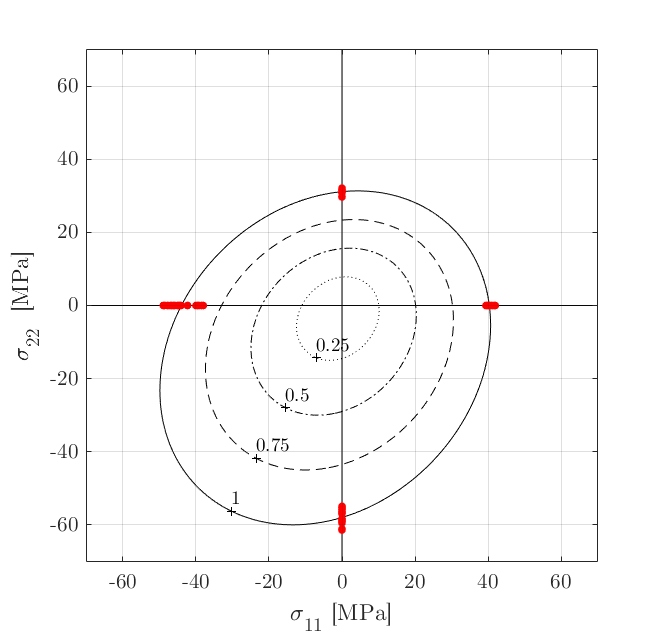
\includegraphics[width=\linewidth, keepaspectratio]{11_22plane}
	\captionsetup{justification=centering} %long caption
	\caption[failure envelope in the $\sigma_{11}$-$\sigma_{22}$ plane]{$\sigma_{11}$-$\sigma_{22}$ plane including data of $X_t$, $X_c$, $Y_t$ and $Y_c$ tests. Graph shows calculated f values of 1, 0.75, 0.50 and 0.25 to illustrate safety factors of 1, 4/3, 2 and 4 respectively} \label{fig:1122plane}
\end{figure}

It can be seen from the tilt of the envelope that there's a strong interaction between the transverse and longitudinal stresses. Computing all tensorial components associated with the  $\sigma_{11}$-$\sigma_{22}$ plane results in Table \ref{tab:1122calc}. Note how $F_{1122}$ is negative and in the same order of magnitude as $F_{1111}$ and $F_{2222}$. 

\begin{table} [h]
	\centering
	\caption{Tensorial components obtained from tests in the $\sigma_{11}$-$\sigma_{22}$ plane}
	\begin{tabular}{ c c } 
		\toprule
		\textbf{Component} & \textbf{Value} \\
		\midrule
		$F_{11}$ & 1.023$\times 10^{-3}$\\ [1ex]
		$F_{1111}$ & 5.663$\times 10^{-4}$\\ [1ex]
		$F_{22}$ & 7.435$\times 10^{-3}$\\ [1ex]
		$F_{2222}$ & 6.095$\times 10^{-4}$\\ [1ex]
		$F_{1122}$ & -3.139$\times 10^{-4}$\\ [1ex]
		\bottomrule
	\end{tabular}
	\label{tab:1122calc}
\end{table}  

Figure \ref{fig:1122plane} indicates that FFF parts produced with the print parameters used should show considerable strengthening when loaded bi-axially in compression. Further experimental work would be of interest to compare bi-axial compression test data to this result.
% Nomenclature introduced in this chapter:
\nomenclature[A]{ADT}{Anderson-Darling Test}% 

% Symbols introduced in this chapter:
%\nomenclature[S]{$\epsilon$}{Engineering Strain \nomunit{$-$}}%
\end{document}